Randomized and approximation
algorithms can obtain significant benefits from coordination directives because although the final
program results will not be exact, they follow important statistical properties and can be computed faster.
Examples of such programs are Loopy Belief
Propagation~\cite{Gonzalez+al:aistats09paraml} (shown in the next section) and
Heat Transfer~(HT).

In HT, we have a graph of nodes that exchange heat values between them. The goal
of the program is to exchange heat to a point where new heat value $\delta = |H_i -
H_{i-1}| \le \epsilon$ for all nodes of the graph. The algorithm works
asynchronously since heat values can be updated by using new partial information
coming from neighbor nodes. This increases parallelism since nodes do not need
to synchronize if we had to compute heat values using iterations.

Fig.~\ref{code:ht} shows the HT logical rules that send new heat values to
neighbor nodes. We added the first rule to increase the priority of the neighbor
nodes if the current node has a large $\delta$. The idea is to prioritize the
computation of heat values of nodes (using \texttt{update}) that have a neighbor
node that changed significantly. Multiple \texttt{add-priority} facts will
increase the priority of a node so that nodes with multiple large deltas will
have more priority. Note that the LM compiler will merge the three rules in
Fig.~\ref{code:ht} into a single one that handles the 3 branches.

\begin{figure}[h!]
\scriptsize\begin{Verbatim}[numbers=left,commandchars=\\\[\]]
new-heat(A, New, Old),
Delta = fabs(New - Old),
Delta > epsilon * 2.0
   -o {B, W | !edge(A, B, W) |
         new-neighbor-heat(B, A, New),
         update(B), \underline[add-priority(B, Delta)]}.

new-heat(A, New, Old),
Delta = fabs(New - Old)
Delta < epsilon * 2.0,
Delta > epsilon
   -o {B, W | !edge(A, B, W) |
         new-neighbor-heat(B, A, New), update(B)}.

new-heat(A, New, Old)
Delta = fabs(New - Old)
Delta < epsilon
   -o {B, W | !edge(A, B, W) |
         new-neighbor-heat(B, A, New)}.
\end{Verbatim}
  \caption{Coordination code for the Heat Transfer program. We added one rule
     that covers cases where $\Delta$ is at least $2 \epsilon$ in order to
     increase the priority of neighbors nodes. The code logic remains exactly
     the same as before, however bigger changes in heat values are now
     propagated faster.}
  \label{code:ht}
\end{figure}
\normalsize

Fig.~\ref{results:ht} presents the scalability results for the uncoordinated
and coordinated version. The dataset used is a square grid with an inner square
with high heat nodes. With 1 thread, there's a 33\% reduction in run time, while
for 16 threads, there's a 18\% reduction.

\begin{figure}[ht!]
   \begin{center}
      \subfloat[]{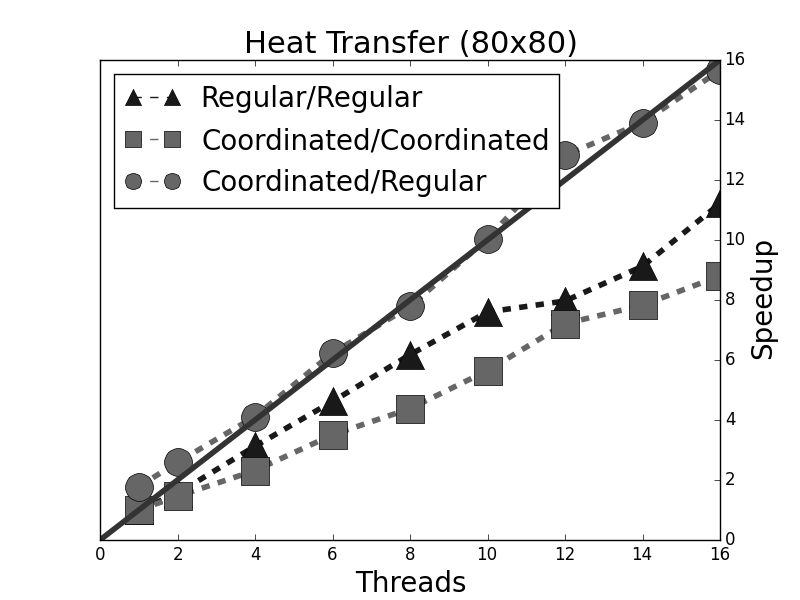
\includegraphics[width=5cm]{results/new-heat-transfer-80}}
   \end{center}
   \caption{Experimental results for the HT program. Speedup values for the
      coordinated and uncoordinated version are computed using the run time of
      the uncoordinated version using 1 thread.}
   \label{results:ht}
\end{figure}
